\def\eurocrypt{1} % set this to 1 for crypt 2012 submission
\def\ccs{0} %set 1 to put in CCS sig alternate style
            %set 0 to put in crypto style

\ifnum\ccs=1
\documentclass{sig-alternate}
\else
\documentclass[12pt]{article}
\usepackage{amsthm}
\fi

\usepackage{amsmath,graphicx,hyperref,xspace,algorithm,color}
\usepackage[noend]{algorithmic}
\def\shownotes{0}   % set 1 for version with author notes
                    % set 0 for no notes

\ifnum\eurocrypt=1
\def\anon{1}
\else
\def\anon{0}   % set 1 to anonymize
                    % set 0 otherwise
\fi

\providecommand{\ie}{\emph{i.e.,} }
\providecommand{\eg}{\emph{e.g.,} }
\providecommand{\cf}{\emph{cf.,} }
\providecommand{\vs}{\emph{vs.} }
\providecommand{\resp}{\emph{resp.} }
\providecommand{\etal}{\emph{et al.} }   %Removed trailing space here; usually want non-breaking space with
\providecommand{\etc}{\emph{etc.}}      % No trailing space here either
\providecommand{\mypara}[1]{\smallskip\noindent\emph{#1} }
\providecommand{\myparab}[1]{\smallskip\noindent\textbf{#1} }
\providecommand{\myparasc}[1]{\smallskip\noindent\textsc{#1} }


\newcommand{\myitem}{\vspace{-.15cm}\item}

\newcommand{\eps}{\epsilon}
\newcommand{\drawn}[1]{\stackrel{#1}{\leftarrow}}
\newcommand{\drawnr}{\drawn{R}}
\newcommand{\defn}{\doteq}
\newcommand{\sign}{\mathrm{sign}}
\newcommand{\bits}{\{0,1\}}
\newcommand{\emty}{\eps}
\newcommand{\hash}{\mathrm{hash}}
\newcommand{\xor}{\oplus }

\newcommand{\Dom}{\text{Domain}}
\newcommand{\Range}{\text{Range}}

\newcommand{\Gen}{\textsf{Gen}\xspace}
\newcommand{\Sign}{\textsf{Sign}\xspace}
\newcommand{\Ver}{\textsf{Ver}\xspace}
\newcommand{\GT}{\textsf{GT}\xspace}
\newcommand{\HT}{\textsf{HT}\xspace}
\newcommand{\HTree}{\textsf{HTree}\xspace}
\newcommand{\Lookup}{\textsf{Lookup}\xspace}
\newcommand{\Add}{\textsf{Add}\xspace}
\newcommand{\SimG}{\textsf{Sim-G}\xspace}
\newcommand{\SimH}{\textsf{Sim-H}\xspace}
\newcommand{\SimS}{\textsf{Sim-S}\xspace}
\newcommand{\FindClaw}{\textsf{FindClaw}\xspace}
\newcommand{\PRF}{\textsf{PRF}\xspace}
\newcommand{\seed}{\textsf{seed}\xspace}


%SPEC STUFF

%\newcommand{\PRF}{\text{PRF}}
\newcommand{\MGF}{\text{MGF}}
\newcommand{\HMAC}{\text{HMAC}}
\newcommand{\RAND}{\text{RAND}}
\newcommand{\RSAGEN}{\text{RSAGEN}}
\newcommand{\RSASIG}{\text{RSASIG}}
\newcommand{\RSAVER}{\text{RSAVER}}
\newcommand{\RSASP}{\text{RSASP}}
\newcommand{\RSAVP}{\text{RSAVP}}
\newcommand{\OStIP}{\text{OS2IP}}
\newcommand{\ItOSP}{\text{I2OSP}}
\newcommand{\BStIP}{\text{BS2IP}}
\newcommand{\ItBSP}{\text{I2BSP}}
\newcommand{\PKF}{\text{PKFingerPrint}}



\newtheorem{theorem}{Theorem}[section]
\newtheorem{task}{Task}[section]
\newtheorem{definition}[theorem]{Definition}
\newtheorem{lemma}[theorem]{Lemma}
\newtheorem{claim}[theorem]{Claim}
%\newtheorem{task}[theorem]{Task}
%

%%%%%%%  Author Notes %%%%%%%
%
\ifnum\shownotes=1
\newcommand{\authnote}[2]{{\marginpar{\color{red} \small #1 notes} $\ll$\textsf{\footnotesize #1 notes: #2}$\gg$}}
\else
\newcommand{\authnote}[2]{}
\fi
\newcommand{\Snote}[1]{{\authnote{Sharon}{#1}}}
\newcommand{\SNOTE}[1]{{\authnote{Sharon}{#1}}}
\newcommand{\Lnote}[1]{{\authnote{Leo}{#1}}}
%%%%%%%%%%%%%%%%%%%%%%%%%%%%%%%%%


\setlength{\topmargin}{-1.2cm}
\setlength{\oddsidemargin}{0cm}
\setlength{\evensidemargin}{0cm}
\setlength{\textheight}{22.9cm}
\setlength{\textwidth}{16.5cm}

\title{Predicting NSF Award Money from Abstracts}
\author{Kyle Brogle \and Sean Ma  \\ Stanford University \and Laura Stelzner}

\begin{document}

\ifnum\ccs=0
\ifnum\eurocrypt=0
\begin{titlepage}
\else
\pagenumbering{arabic}
\fi
\else
\pagenumbering{arabic}
\fi

\maketitle

%\begin{abstract}
%\medskip\noindent
%\textbf{Keywords:} Text classification, Naive Bayes, SVM, Softmax Regression
%\end{abstract}

\ifnum\ccs=0
\ifnum\eurocrypt=0
\end{titlepage}
\tableofcontents
\newpage
\fi
\fi

\section{Introduction}

The National Science Foundation is the gatekeeper of  billions of dollars used for scientific research in the United States.  This funding is critical to making advancements in science, mathematics, and other related fields such as medicine.  In 2012 the NSF received 7.033 billion dollars of funding (http://www.nsf.gov/about/congress/112/highlights/cu11\_1118.jsp), most of which will be allocated to distribution of research awards to researchers.   As mentioned from the NSF funding description page, “NSF receives approximately 40,000 proposals each year for research, education and training projects, of which approximately 11,000 are funded.” (http://www.nsf.gov/funding/aboutfunding.jsp).   We used machine learning techniques to classify the amount of funding a NSF proposal would receive based on past funding allocations.  Reviewing 40,000 proposals by hand takes a lot of time.  Initial data from machine learning could help speed the process by helping determine which proposals are most promising given what they’ve awarded in the past, and the classifier can continually be adjusted over the years as more proposals are available as training data.

\section{Data}

\begin{figure*}[h]
\centering
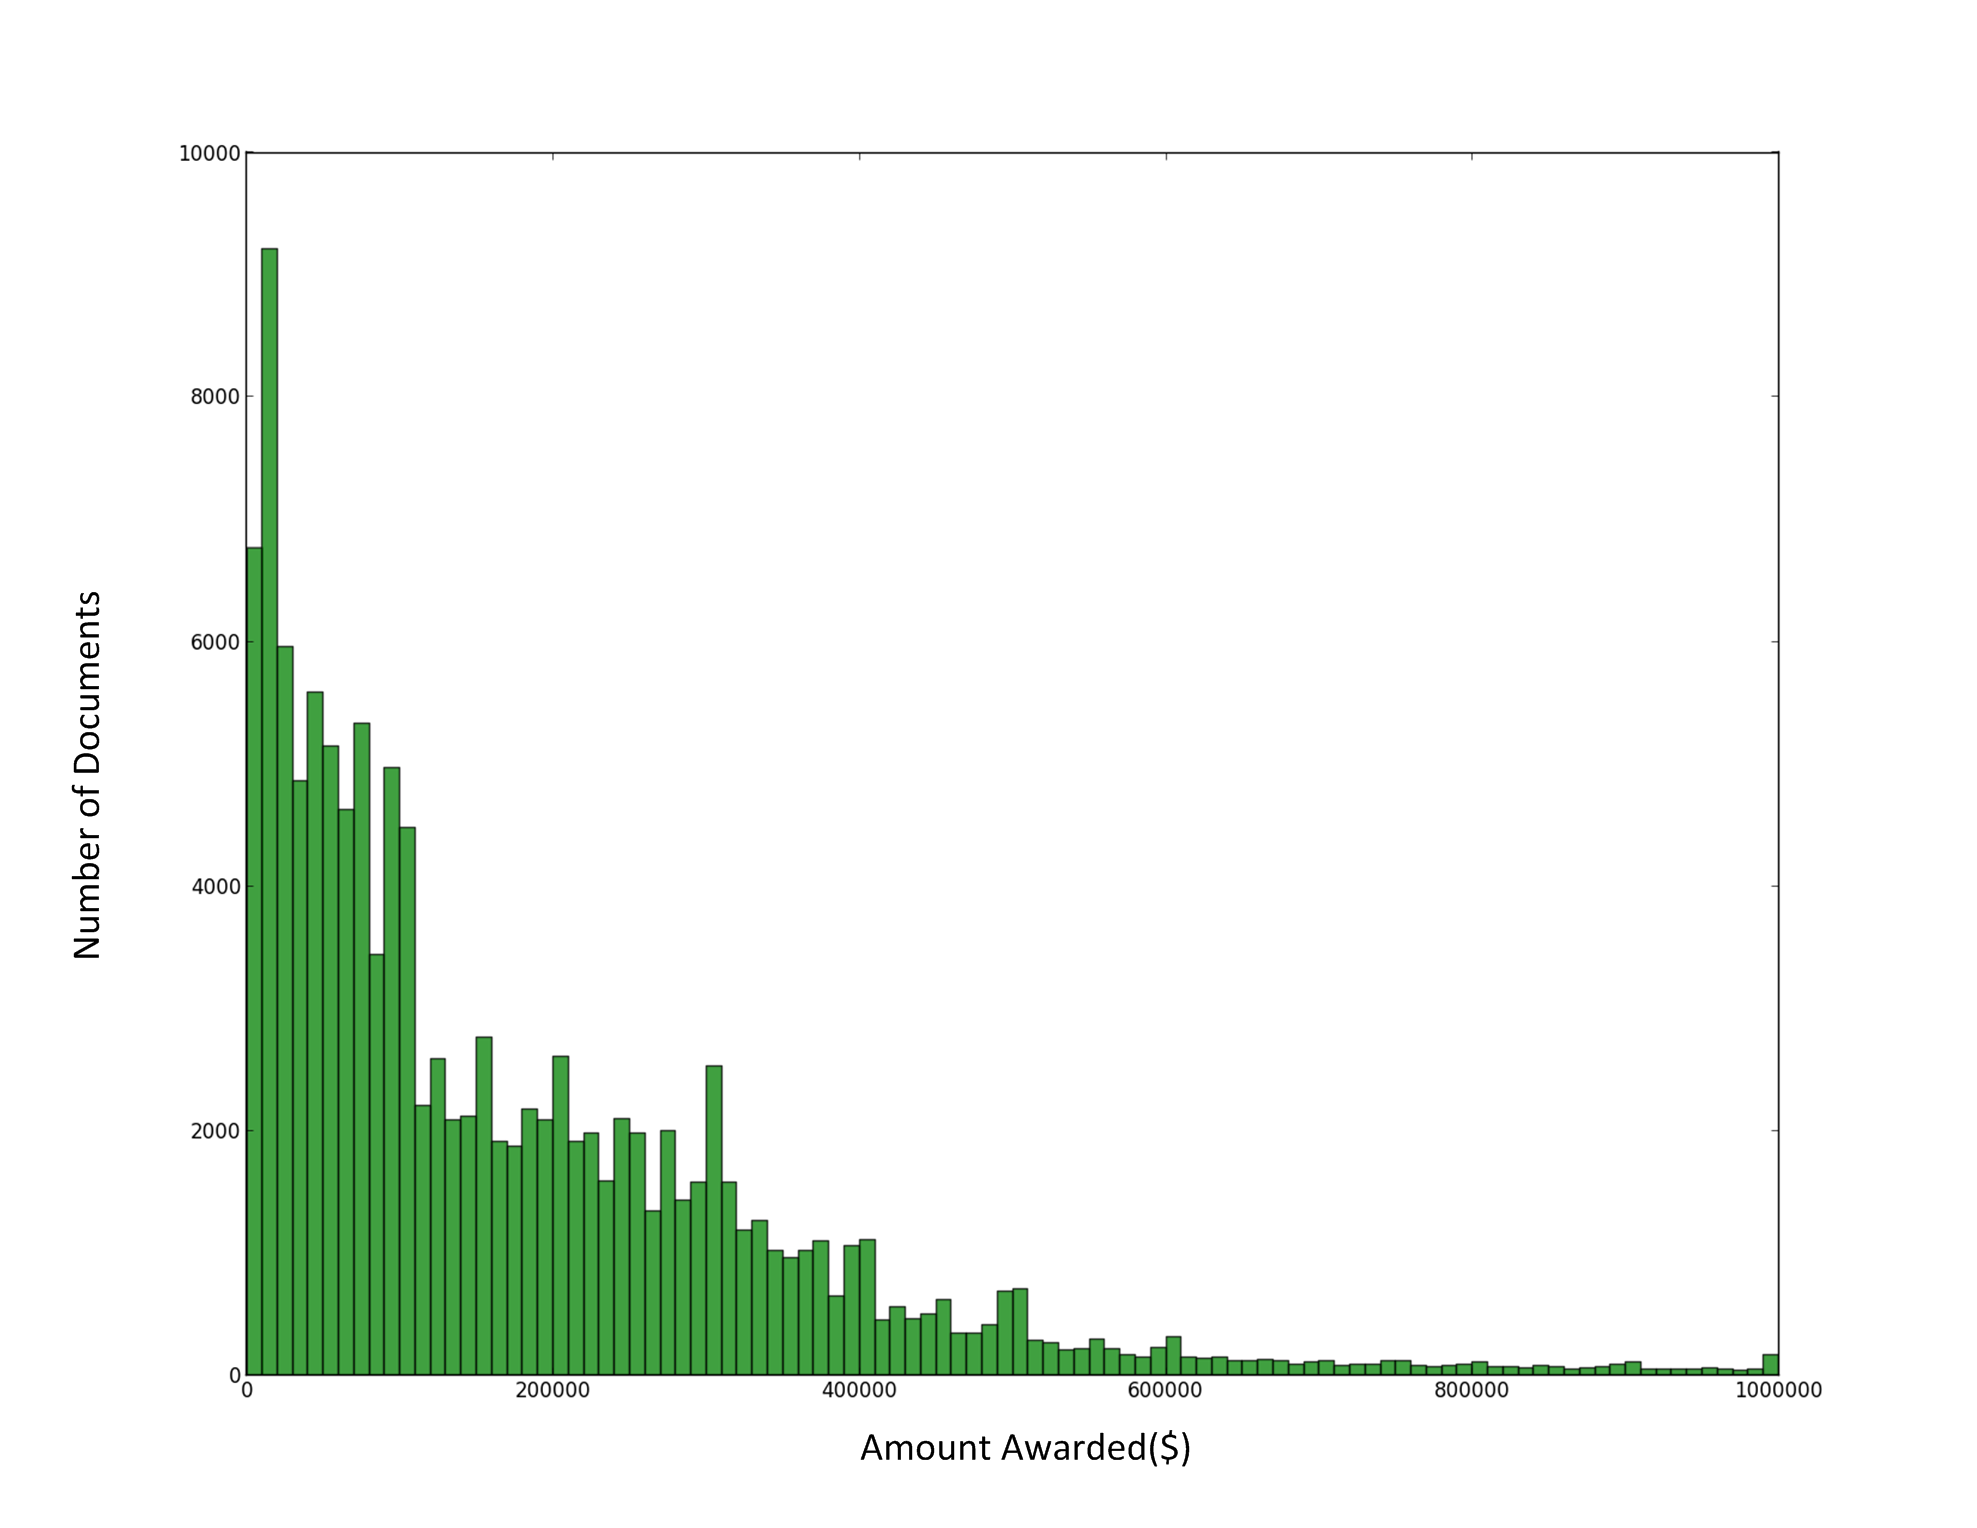
\includegraphics[width=100mm]{histo_pretty.png}
\caption{A histogram detailing a relative distribution of how the data is distributed}
\end{figure*}

For our data we have 129,079 proposals submitted to the NSF between 1990 and 2003 courtesy of University of California, Irvine’s Machine Learning Repository. We began by giving each proposal a unique identifier. The proposals were all parsed into a bag-of-words format in order to transform them into feature vectors to be classified.  We removed stop words from our vocabulary, as they are too common in occurrence to aid in classification.  Our dictionary of words produced was of length 30,799.  We also extracted the awarded amounts from the proposals themselves.  An initial histogram of the training data suggested that 21 class labels would nicely divide the proposals: twenty buckets in increments of \$50,000 up to \$1 million, and one bucket for awards greater than \$1 million.

\section{Method and Results}

After our data was processed into a usable format, we decided to start by training a multi-class SVM with linear kernel to classify our data.  Although we have approximately 130,000 training examples, we trained on smaller subsets.  In order to determine whether the size of the training set impacted our classification error, we decided to train the SVM with training set sizes 1000, 2000, 5000, and 10000.  These sets were built by randomly choosing documents from our dataset, to try to avoid training sets that are similar in topic or year requested.  In each training scenario, we used 5-fold cross-validation in order to test the accuracy of our model.  When analyzing the results, we found that the linear SVM suffers from extremely high variance, as our training error is near zero.  In order to try and remedy this, we decided to simplify our model by reducing the number of features.  In order to do this, we reduced the vocabulary size by using the Porter2 stemming algorithm to stem all the words in our vocabulary.  This reduced vocabulary size from 30,799 to 19,910.  This resulted in less overfitting of our model, but the high variance persisted.  Before spending time training on larger training sets, we decided to investigate the performance of some other classifiers. \\

\begin{figure*}[h]
\centering
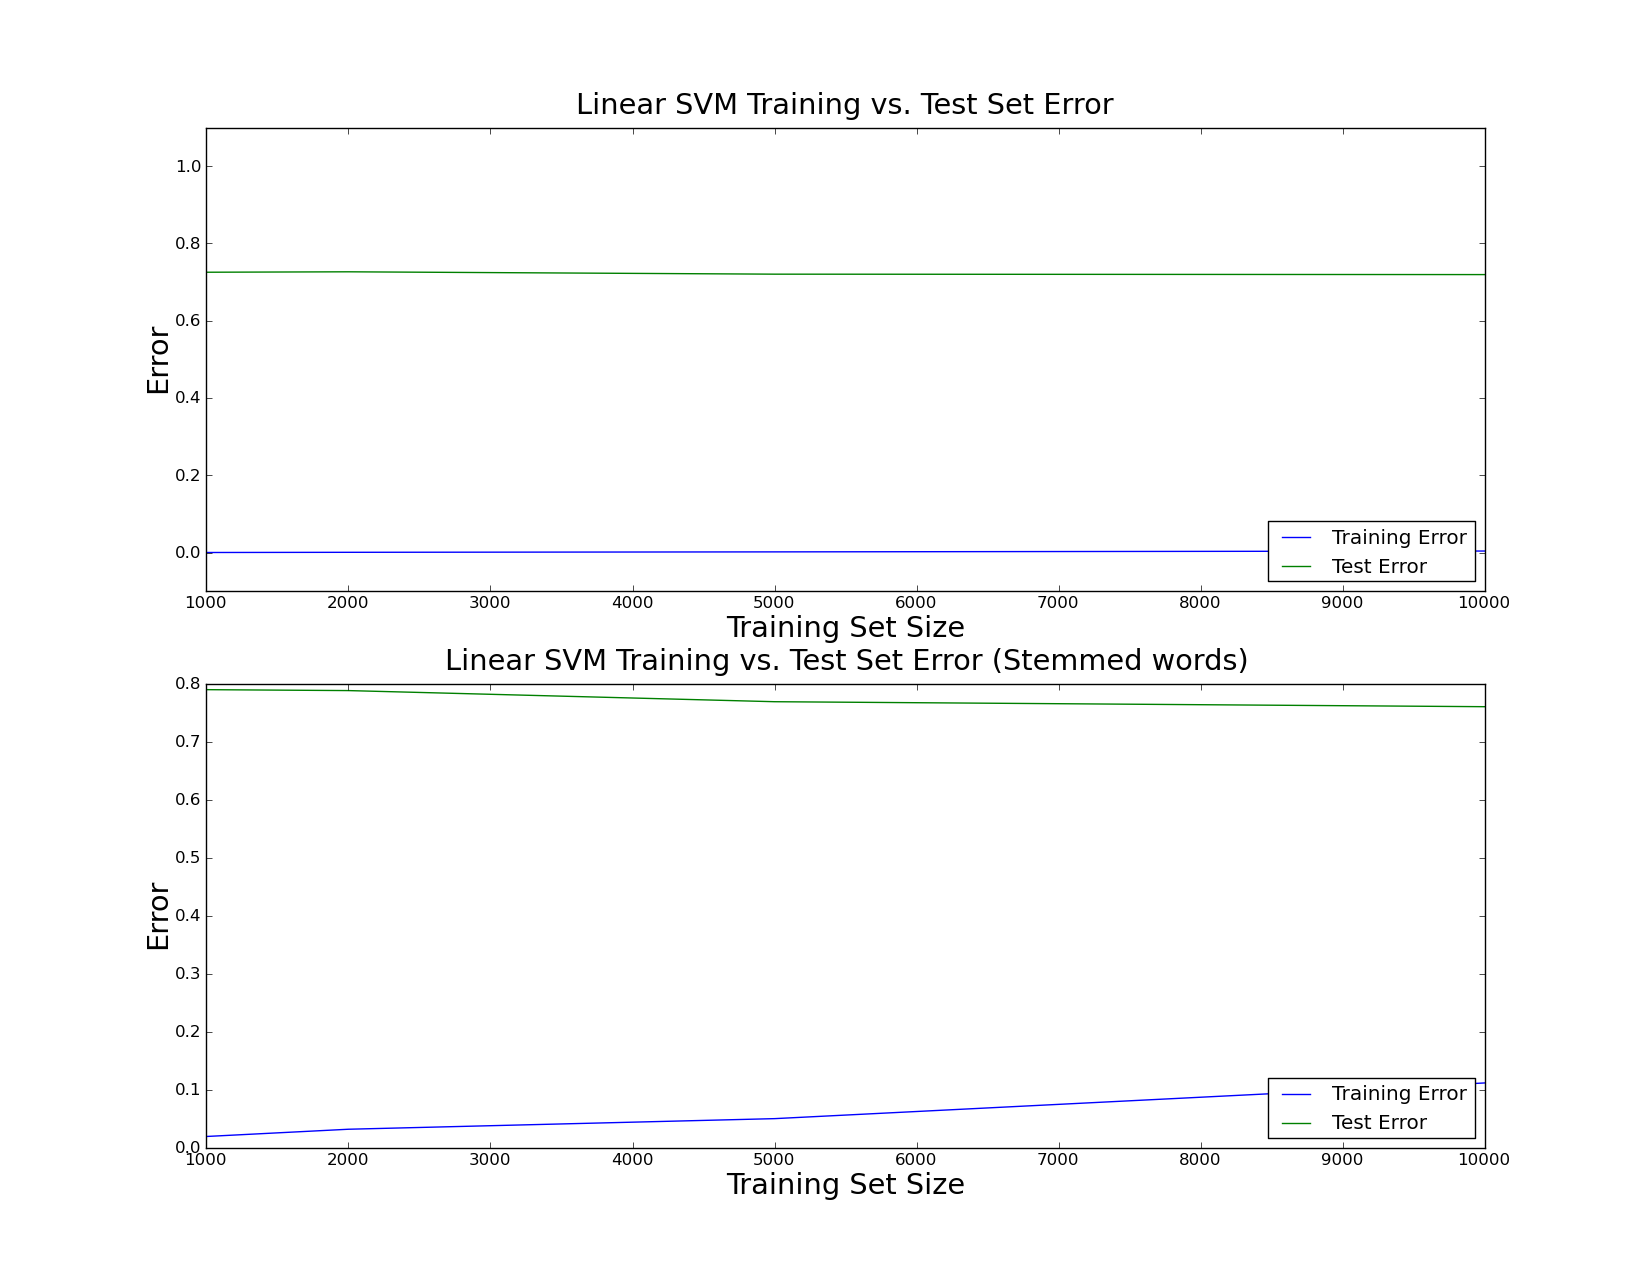
\includegraphics[width=150mm]{linsvm_train_vs_test_both.png}
\caption{Training vs. Test Error for Linear SVM}
\end{figure*}

The additional classifiers we chose to test were multinomial Naive Bayes, and Stochastic Gradient Descent.  We then ran these classifiers on both the stemmed and non-stemmed training sets of sizes 1000, 2000, 5000, and 10000.  The Naive Bayes classifier seemed to perform the best of all our classifiers, exhibiting classification accuracy of 33 percent.  With 21 classes, the trivial classifier that uniformly selects a class for each document would achieve 4.8 percent accuracy if the distribution of classes over documents was uniform.  It would actually achieve less in this application, since the documents are concentrated in categories with lower award amounts.  We found that the training error was also high (around 40 percent), indicating high bias.  Because of the high bias, the reduction of the feature space provided by the stemmed dataset caused Naive Bayes to perform extremely poorly. \\

\begin{figure*}[h]
\centering
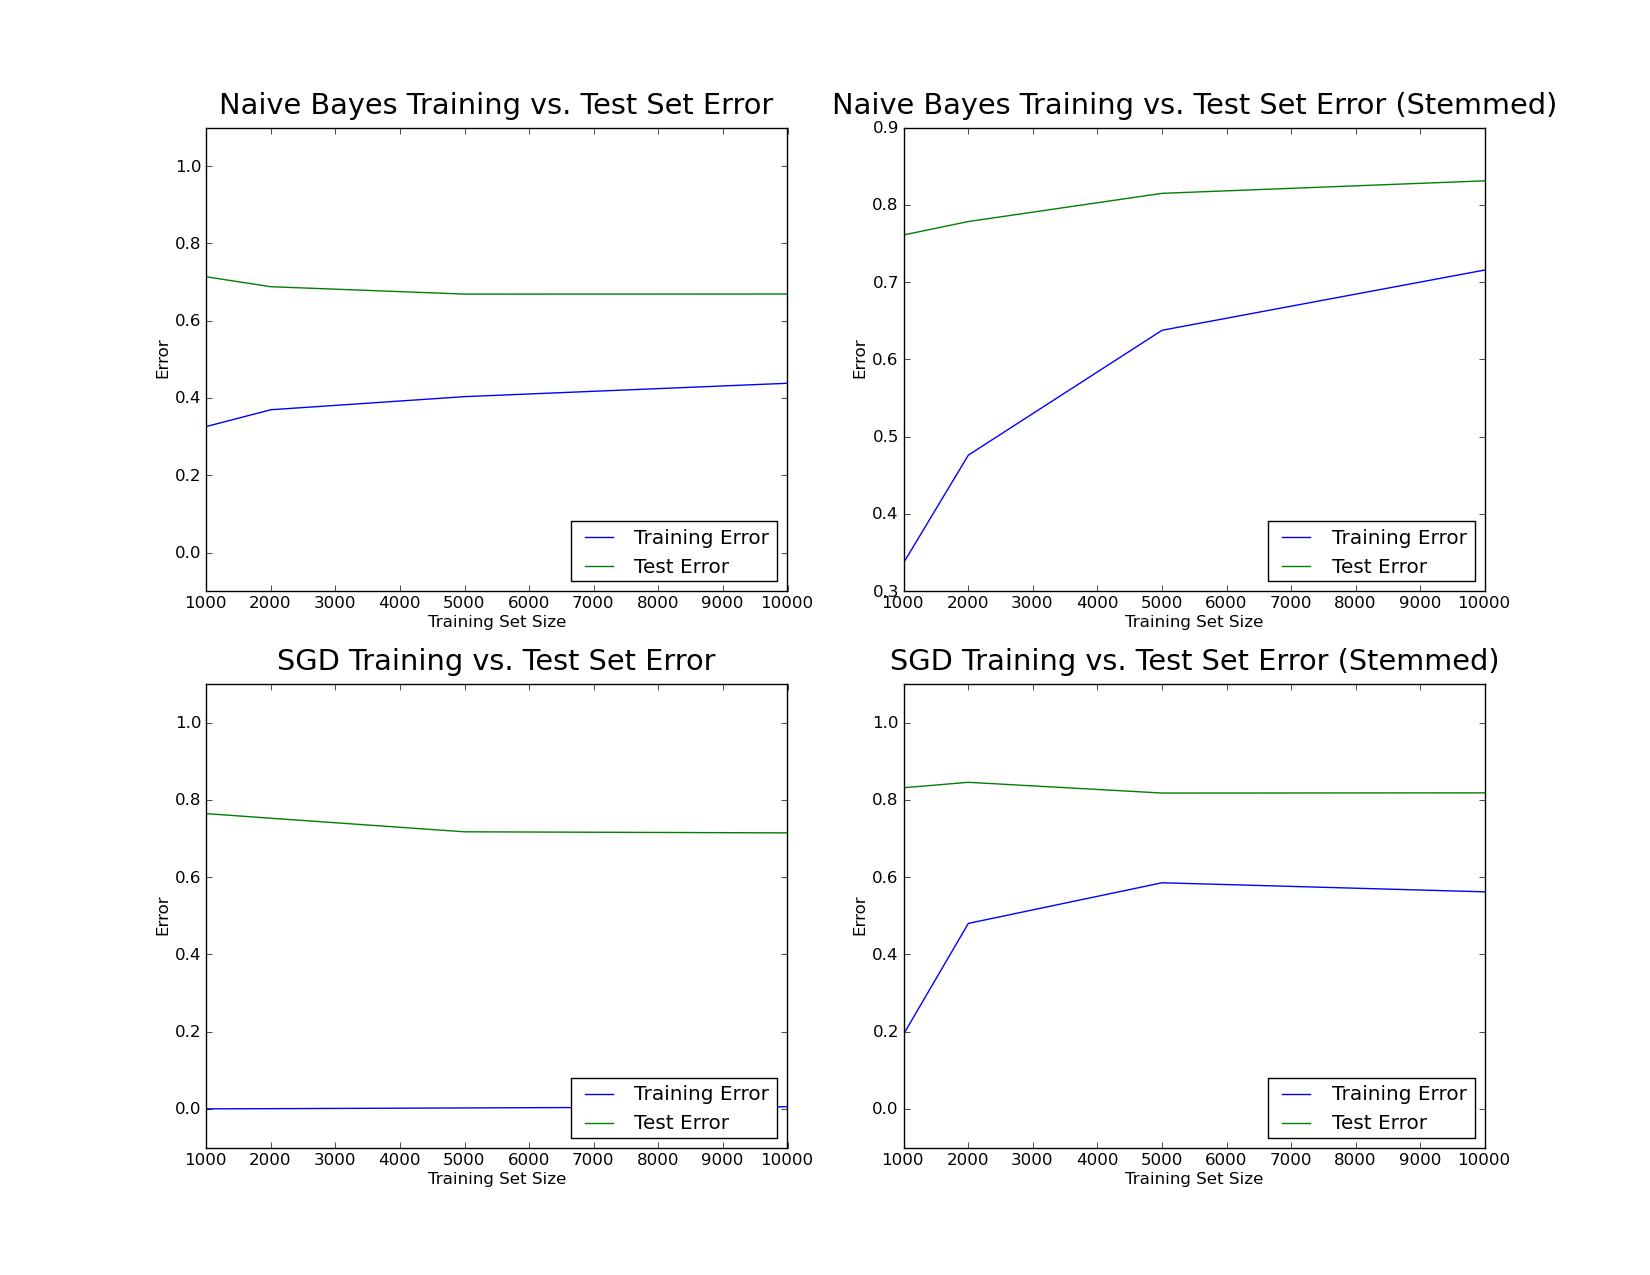
\includegraphics[width=150mm]{other_train_vs_test_both.png}
\caption{Training vs. Test Error for Naive Bayes and Stochastic Gradient Descent}
\end{figure*}

On the other hand, when using a stochastic gradient descent classifier, we found classification accuracy to be around 28 percent.  Like the linear SVM, this classifier had very small training error, due to overfitting the model to the training set.  When training on the stemmed dataset, the reduced feature set had a more significant impact here than with the linear SVM.  With the reduced feature set, the classifier no longer overfit the model to the training data, and started to exhibit signs of high bias.  The accuracy of our classifications decreased when running on the stemmed data in this scenario.


\section{Conclusions}
From our analysis, we see that the best performance was realized with the Naive Bayes classifier on the un-stemmed dataset.  Unlike the linear SVM and stochastic gradient descent classifiers, Naive Bayes did not overfit our model to the training set.  The high training error in Naive Bayes indicates high bias, which suggests that classification error can be lowered with the addition of more features to the model.

\section{Future Work}
In order to further improve the accuracy of the Naive Bayes classifier, we plan to address the high bias by adding more features.  One specific feature that we feel will improve the classification accuracy greatly is the year of submission.  This should really be considered in our model, as popular research areas, especially in the field of computer science, tend to change over time, with new topics emerging frequently.  This feature will be weighed much higher than the bag of words features, as we suspect it plays a significant role in funding decisions.  Other features that were suggested to us during poster presentations were the sponsoring university and the department, which we could infer from either the principal investigator’s mailing address or the NSF program ID.\\

We also wish to extend the dataset by contributing proposals up to the current year.  We are currently writing a script to parse the award format provided by the NSF awards website.

\section{Citations}
\noindent
[1] Frank, A. \& Asuncion, A. (2010). UCI Machine Learning Repository [http://archive.ics.uci.edu/ml]. Irvine, CA: University of California, School of Information and Computer Science. \\ \\
\noindent
[2] National Science Foundation.  About Funding. In {\it National Science Foundation Where Discoveries Begin}. Retrieved Nov 15, 2012, from http://www.nsf.gov/funding/aboutfunding.jsp \\ \\
\noindent
[3] National Science Foundation. FY 2012 Appropriations Signed Into Law--NSF to Receive \$7.033 Billion. In {\it National Science Foundation Where Discoveries Begin}. Retrieved Nov 15, 2012, http://www.nsf.gov/about/congress/112/highlights/cu11\_1118.js\\ \\
\end{document}
